\documentclass[../../main.tex]{subfiles}
\begin{document}

\subsection*{1.3}
Quattro cariche puntiformi di egual valore $q = 10^{-8}C$ sono poste ai vertici di un quadrato di lato a = 10 cm. 
\\Calcolare l’energia potenziale elettrostatica del sistema e il lavoro necessario per spostare una delle cariche dalla posizione iniziale P1 al punto P2 indicato in figura e situato nel centro del lato.
\\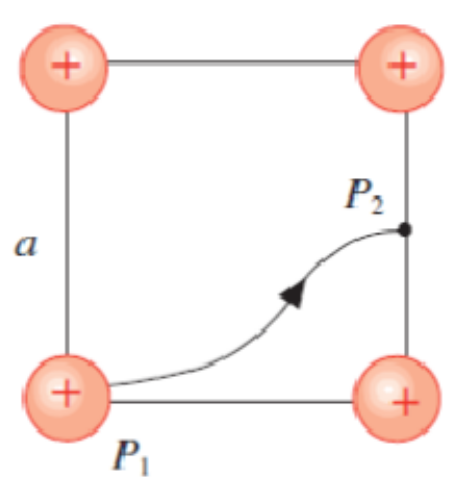
\includegraphics[scale=0.3]{e_1_3.png}
\subsubsection*{Formule utilizzate}
$U_e[P] = \frac{1}{2}\sum_{i \ne j}\frac{q_i\ q_j}{4\pi \epsilon_0 r_{ij}}$
\\$W = U_e[P_2] - U_e[P_1]$
\subsubsection*{Soluzione}
$U_e[P_1] = \frac{1}{2}\sum_{i \ne j}\frac{q_i\ q_j}{4\pi \epsilon_0 r_{ij}} = \frac{2q^2}{4\pi\epsilon_0a}\left(2 + \frac{1}{\sqrt{2}}\right) = 4.87 * 10^{-5}\ J $
\\$U_e[P_2] = \frac{q^2}{4\pi\epsilon_0a} \left(2+ \frac{1}{\sqrt{2}}\right) = 6.84 * 10^{-5}\ J$
\\$W = U_e[P_2] - U_e[P_1] = 1.97 * 10^{-5}\ J $
\newpage

\end{document}